\documentclass[a4paper,10pt,conference]{ieeeconf}  

\IEEEoverridecommandlockouts                             

\overrideIEEEmargins                                   

\usepackage{amsmath}
\usepackage{amsfonts}
\usepackage{graphicx}
\usepackage{color}


\title{\LARGE \bf Control Engineering: Maximizing Performance of the Fourth-Order Motion Setup (or any other title you fancy)}

\author{\textcolor{red}{$<$ NAMES, STUDENT NUMBERS AND TEAM NUMBER $>$} }% 
\begin{document}

\maketitle 
\thispagestyle{plain}
\pagestyle{plain}


\section{\textbf{Introduction}}

\textcolor{red}{You have been given the assignment to obtain an as good as possible tracking performance of the Fourth-Order Motion Setup, depicted in Fig.~\ref{fig:example}, using feedback and/or feedforward techniques, according to the assignment described in `Exercise X'. Use this article template to document your approach and results.
	\begin{itemize}
		\item Clearly describe your performance measure and control objective, methods you've used, motivation for your controller design, the obtained performance, the measurements you performed, the lessons you've learned, etc. in a concise and condense manner.
		\item Make use of figures and plots to make your points, explain your reasoning, proof your claims and motivate your choices.
		\item Limit yourself to max 6 pages! Every additional page will cost you 0.5 points on your report grade. Not using this template at all will cost you 1.5 points. Your final grade for the course will be a weighted combination of your report grade and Canvas quiz grade.
		\item This document has to be submitted as a single PDF via Canvas before the deadline (see the Assignments section).
		\item Feel free to modify the predefined structure below if you don't agree, or think you can do better.
	\end{itemize} }

%%%%%%%%%%%%%%%%%%%%%%%%%%%%%%%%%%%%%%%%%%%%%%%%%%%%%%%%%%%%%%%%%%%%%%%%%%%%%%%%
\section{\textbf{System Identification}}

Fig.~\ref{fig:example} is a reference to an example figure, with a caption below the figure. Remember to let figures float to either the top or bottom of the column.

\begin{figure}[b]
\centering
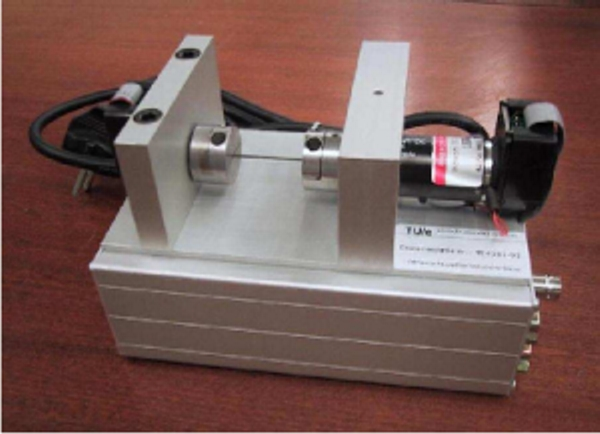
\includegraphics[width=0.9\linewidth]{FORCE.jpg}
\caption{An example figure.}
\label{fig:example}
\end{figure}


%% ====================================================== %%
\newpage

\section{\textbf{Controller design}}

An equation like
\begin{equation}\label{eq:emc}
  E=mc^2,
\end{equation}
where $m$ is the mass and $c$ is the speed of light, is always part of a sentence. Obviously, \eqref{eq:emc} is a legendary equation.


%% ====================================================== %%

\section{\textbf{Experimental results}}

Think about what your main result is; what figure, table or formula will blow the reviewer off his/her chair? If you use a table like Table~\ref{tab:goodbad}, it should of course also float to the top or bottom of a column, with a caption above it.

\begin{table}
\centering
\caption{A dummy table.}
\label{tab:goodbad}
\begin{tabular}{|c|c|c|}
\hline
& $S<1$ & $S>1$ \\
\hline
Verdict & Good & Bad \\
\hline
\end{tabular}
\end{table}

%% ====================================================== %%
\section{\textbf{Conclusions \& Discussion}}
Don't forget to conclude your work.


\section*{\textbf{References}}
Add references if you've used any, e.g. using \textsc{Bib}\TeX.

\end{document}
